\documentclass[12pt,a4paper]{article}

\usepackage{mathtools}
\usepackage{minted}
\usepackage{txfonts}
\usepackage{xcolor}
\usepackage{geometry}
\usepackage{graphicx}
\usepackage{wrapfig}
\definecolor{LightGray}{gray}{0.9}
\graphicspath{ {./images/} }
\geometry{
a4paper,
left=20mm,
right=20mm,
top=20mm,
bottom=20mm
}

\title{Nutrient Analysis}
\author{Alex Viller, 45375325}
\date{}

\begin{document}
    \maketitle

    \tableofcontents{}

    \clearpage
    \section{Data Cleaning and Analysis}
    \subsection{Initial Checks}
    The Nutrient information file is a spreadsheet of different nutritional
    information. For this report I have analyzed the "All solids \& liquids per
    100g" sheet. In this sheet, there are 295 features and 291 classes. Upon
    looking through the features I can see that there are features looking at
    the same things, but with different units, i.e. C4 (\%T) vs C4 (g). I chose to
    drop the \%T versions of these data points as they are just a function of
    the grams. I also dropped the food names and public food key columns as these
    were text based datapoints that individually classified every data point.
    \\
    \\
    After some analysis of the classifications column, I noticed that the
    classifications seemed to be tiered. That is the first number was an overarching
    class, then the next number added more specificity, and so on. I went to the
    website that the datasets were gotten from and found a spreadsheet that mapped
    each classification number to what it represented, including each tier of class.
    So I used this spreadsheet to create a mapping. And also having noticed the tiering,
    I filtered the dataset using regex in order to only hold onto either the first 2
    characters of the classifications. Allowing me to reduce the number of classes,
    making classification easier.
    \\
    \\
    These initial transformations resulted in having 293 features and 23 classes. I then
    looked at the values held within the spreadsheet and noticed a lot of the data was
    not filled. So I did a pass through to drop all features where more than 95\% were
    na values. Bringing the number of features down to 60, and a class column, meaning
    61 total columns. We can see a correlation matrix of the remaining classes and features
    in figure \ref{fig:corrmat}
    \begin{figure}[H]
        \caption{Correlation Matrix of Nutrient File after dropping}
        \centering
        \label{fig:corrmat}
        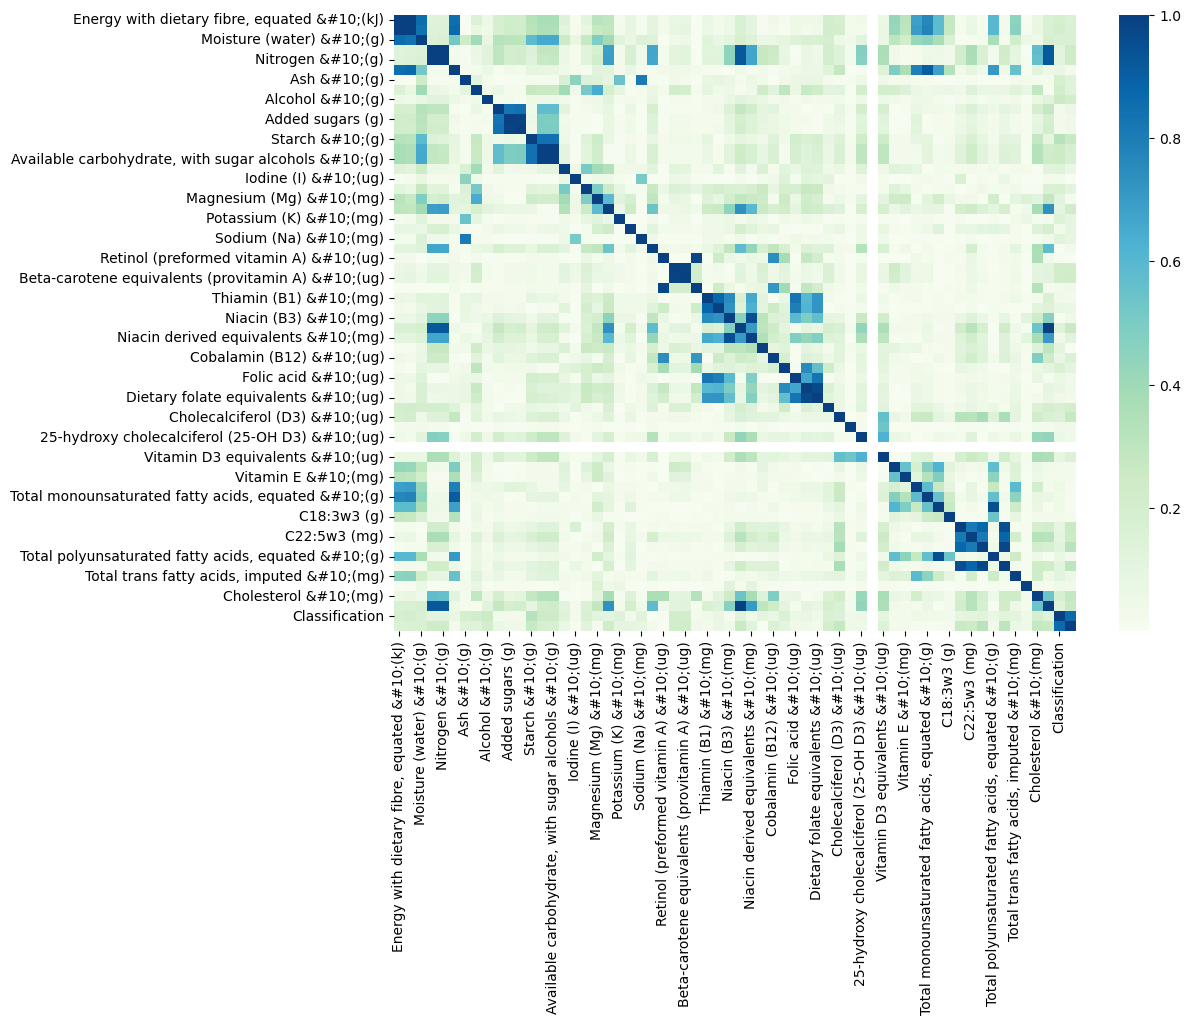
\includegraphics[width=0.85\textwidth]{nopca_heatmap}
    \end{figure}

    \subsection{SMOTE}
    I then noticed that there was a severe class imbalance. Namely, the meat class had
    roughly 450 datapoints, whereas some of the other classes had only 1 or 2. I chose
    to address this imbalance by using imbalanced learns SMOTE library to increase the
    number of points for each class up to the maximum number of datapoints for a class.
    In order to use SMOTE, you require at least k datapoints, where k is the nearest
    neighbours you choose to use. I chose to do 5 nearest neighbours. So I dropped all
    classes that had less than 20 datapoints. This was to hopefully avoid smote just
    copying each datapoint until we had reached the right value.
    \\

    \begin{figure}[h]
        \caption{Code to apply smote}
        \centering
        \label{fig:smotecode}
        \begin{minted}
            [
            frame=lines,
            framesep=2mm,
            baselinestretch=1.2,
            bgcolor=LightGray,
            fontsize=\footnotesize,
            linenos
            ]
            {python}
smote = SMOTE(random_state=42, k_neighbors=5)
X_train, y_train = smote.fit_resample(X_train, y_train)
        \end{minted}
    \end{figure}

    
    The way that SMOTE is implemented in the imbalanced learn library, it makes a
    random sample of other things that fit this class. It then selects its nearest k
    neighbours and generates each feature based on the most common feature nearby.
    \\
    \\
    After the SMOTE is applied, we can see minimal change to the correlation matrix
    as can be seen in figure \ref{fig:postsmotecorrmat} which is to be expected.
    If we saw any big changes we should worry about what SMOTE has done to our data
    to introduce or remove any correlations. We mostly just see already present correlations
    get slightly stronger.

    \begin{figure}[h]
        \caption{Correlation Matrix of Nutrient File after SMOTE application}
        \centering
        \label{fig:postsmotecorrmat}
        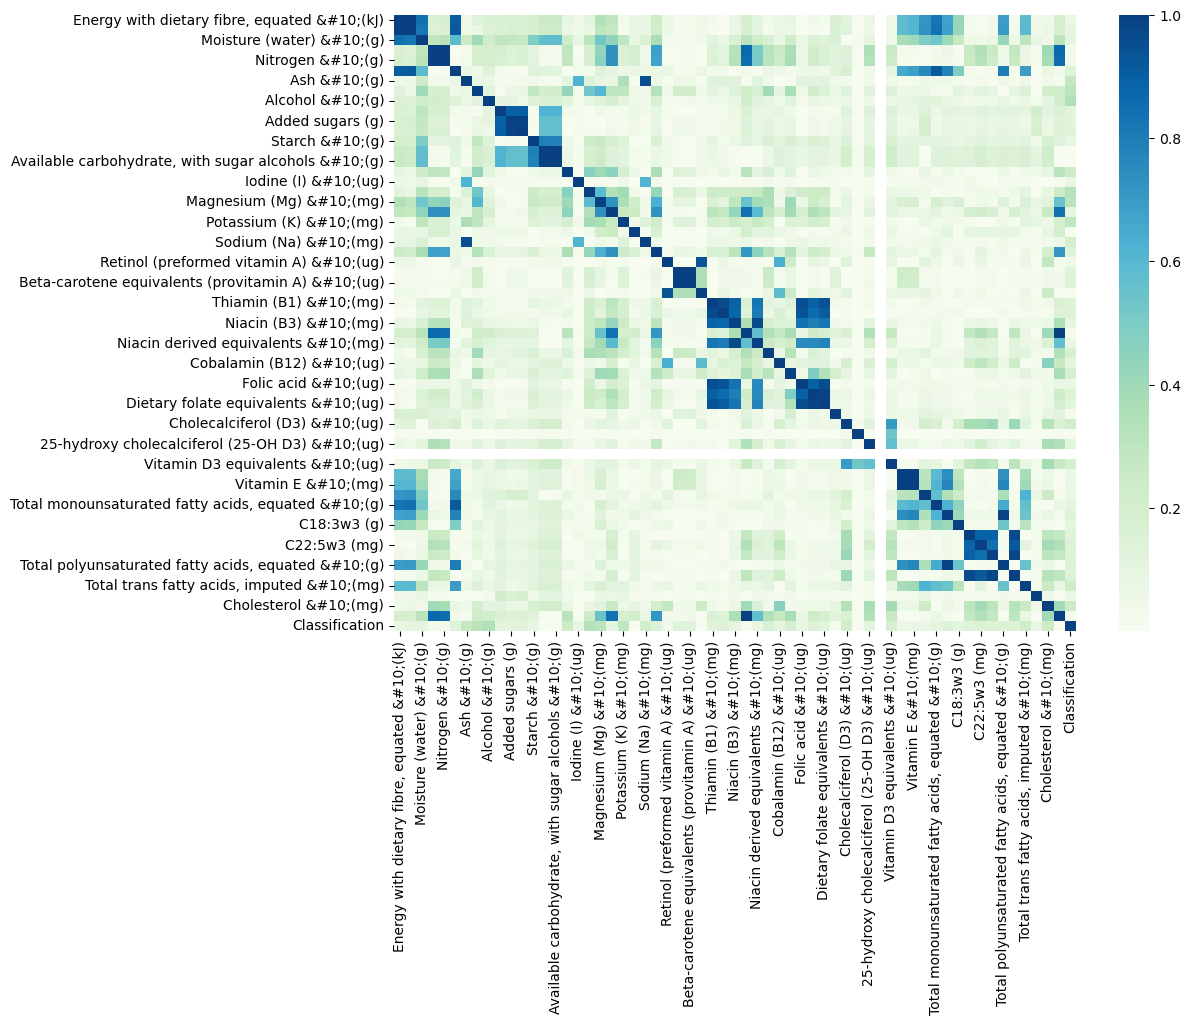
\includegraphics[width=0.78\textwidth]{nopca_postsmote_heatmap}
    \end{figure}

    As I wanted to test the dataset to start with using some simpler techniques such
    as KNN and Random Forest classifiers, I made sure to only apply smote to the train
    data. This is because KNN and Random Forests can become confused by the whole dataset
    having been smoted.

    \subsection{Principal Component Analysis}
    We can consider the use of principal component analysis (PCA) here as well. This is a technique
    which uses a singular vector decomposition of the data in order to project the data into a lower
    dimensional space. This means we need to scale the data beforehand, meaning that the data in each
    feature gets normalized between 1 and 0, with 1 being the old max value, and 0 being the old min 
    value. I will compare its use vs non use throughout the rest of the report.
    \\
    For now, we can see the difference in correlation matrices as well as the explained 
    variance ratio to help choose how many features to use.

    \begin{wrapfigure}{r}{0.35\textwidth}
        \centering
        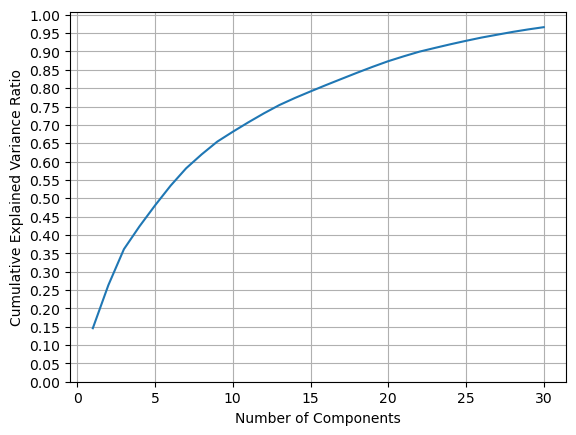
\includegraphics[width=0.4\textwidth]{PCA_variance_ratio}
    \end{wrapfigure}

    With 30 features chosen for PCA, we get the explained variance ratio in the figure to
    the right. 
    \\
    \\
    As we can see, we have stopped right after hitting the 0.95 mark. We interpret this graph
    as seeing that we are explaining 95\% of the data held within our 60 features, using only
    30.
    \\
    \\
    So we have managed to reduce out dimensionality again, giving us data that is once again
    easier to work with. However, this also highlights the importance of these features. As
    for a 1 dimensional problem (In that a 1d array of features points to a single class)
    30 features is a lot to be working on. This blends into an issue of high dimensionality,
    especially when dealing with models like KNN and Random Forests as we will get into later.

    \begin{wrapfigure}{l}{0.45\textwidth}
        \centering
        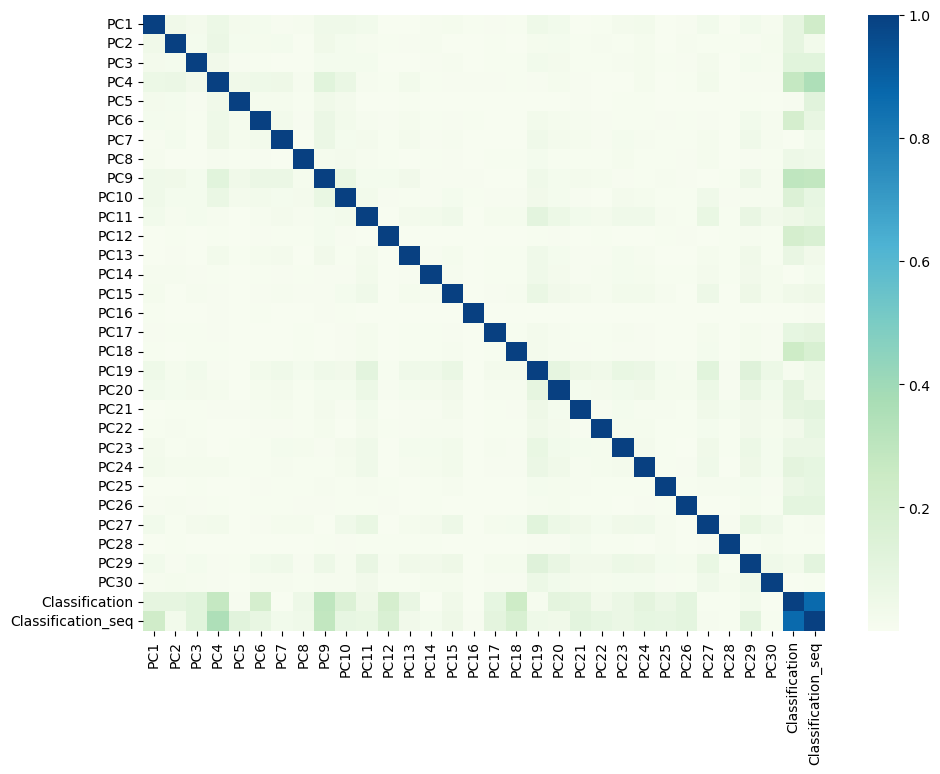
\includegraphics[width=0.4\textwidth]{pca_heatmap}
    \end{wrapfigure}
    
    For now though, we can look at the correlation matrix for our PCA features, to the left.
    We can see that there are stronger relations along the classifications axes.
    \\
    \\
    The 'Classification\_seq' column is identical to the 'Classification' column, except the
    classes have been mapped to be sequential numbers. This is for use later on in some other
    models, otherwise the data is identical. Hence, the near 1 correlations between them.
    \\
    \\

    \begin{wrapfigure}{r}{0.45\textwidth}
        \centering
        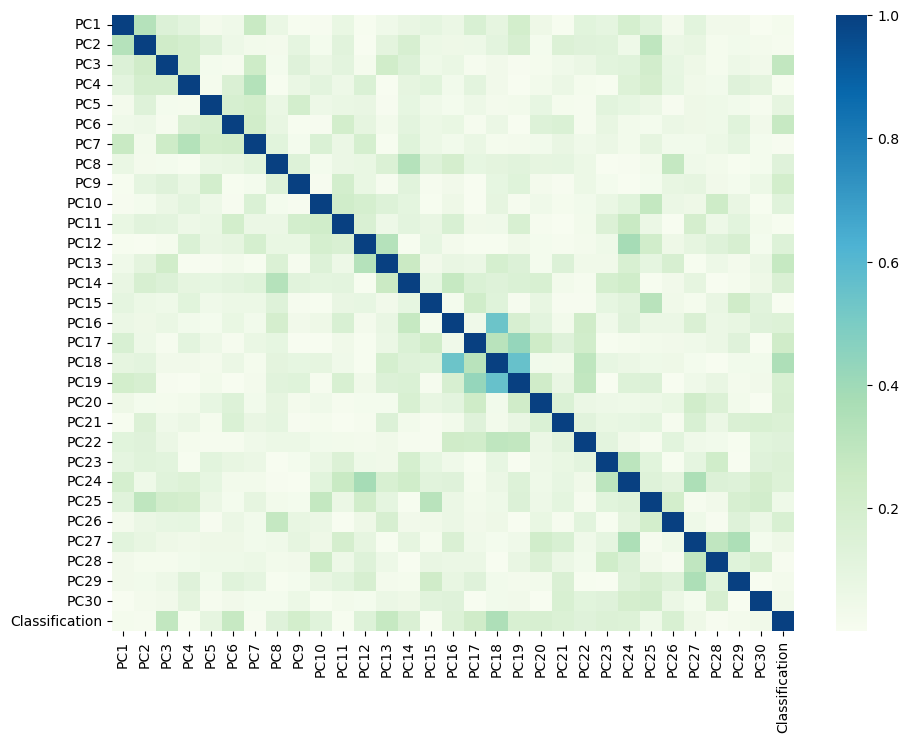
\includegraphics[width=0.4\textwidth]{pca_postsmote_heatmap}
    \end{wrapfigure}

    When we then apply SMOTE to the training set. We see in this correlation matrix far greater
    correlations, not only between the features and the classes, but between the features themselves.
    \\
    \\
    We can notice that all of these correlations were there prior to the smote. However, the SMOTE
    has made them significantly more pronounced.

    \clearpage
    \section{K-Nearest Neighbours Classifier}
    \subsection{Training}
    K-Nearest Neighbour (KNN) classification for a multiclass problem such as this works on a 1 vs. rest
    approach. For each datapoint we look at our nearest neighbours up to k. The closeness of the neighbour
    is calculated through the n dimensional space to find the vector connection with the smallest magnitude.
    \\
    \\
    Interestingly, as we can see below in figures \ref{fig:knn-nopca} and \ref{fig:knn-pca} that as we 
    increase the number of neighbours, the accuracy of our KNN classifier actually gets worse. Typically,
    one would expect that as you increase the depth with which you look at all the different neighbours,
    you also can learn more about what tells you about what class to look at. And even when we reduce the
    dimensionality with PCA we see a very similar graph.

    \begin{figure}[h]
        \centering
        \begin{minipage}{0.45\textwidth}
            \centering
            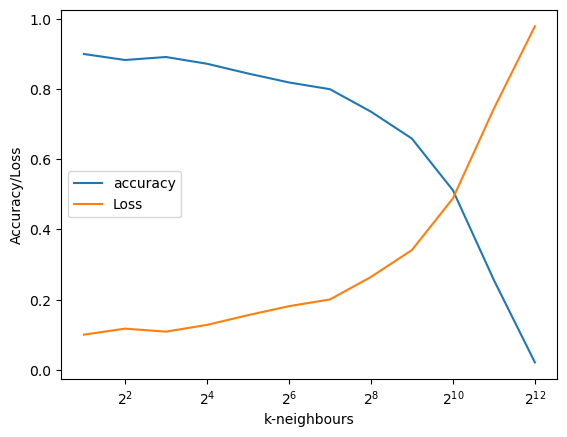
\includegraphics[width=0.9\textwidth]{knn-nopca} % first figure itself
            \caption{KNN model test loss and accuracy vs k. No PCA}
            \label{fig:knn-nopca}
        \end{minipage}\hfill
        \begin{minipage}{0.45\textwidth}
            \centering
            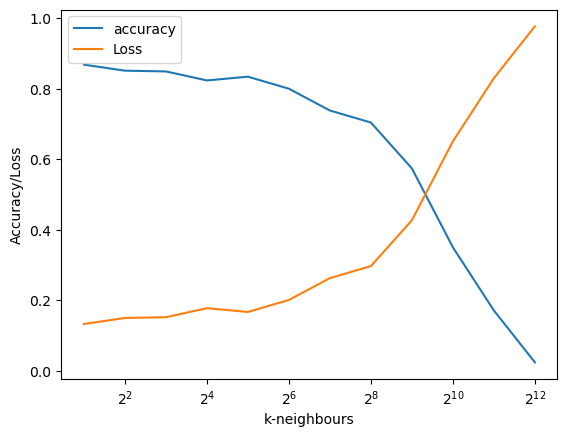
\includegraphics[width=0.9\textwidth]{knn-pca} % second figure itself
            \caption{KNN model test loss and accuracy vs k. Using PCA}
            \label{fig:knn-pca}
        \end{minipage}
    \end{figure}

    I think this is due to, despite lowering the dimensionality of the problem with PCA, we still have
    30 dimensions for KNN to attempt to decipher. This is a very high dimensionality, so attempting to
    find the nearest $2^{12}$ neighbours is very likely to confuse the model, which is why we see our
    best accuracy when we have 4 neighbours, giving us an accuracy of 0.87.

    \subsection{Results}
    We can then observe the precision recall curves in figure \ref{fig:knn-precision-recall},
    and we see that our model has a very high precision for 0 recall, but then
    almost no precision afterwards. This leads us to see that whilst we achieved high accuracy, our model
    is struggling when comparing unseen inputs.
    \\
    \\
    When we compare the confusion matrices for this model in figures \ref{fig:knn-conf-nopca} and \ref{fig:knn-conf-pca}
    we can see, interestingly, that our model that uses PCA, whilst getting its highest accuracy with
    fewer neighbours, has a lower overall accuracy. This confusion matrix also highlights the extreme
    class imbalance within this dataset. This helps explain why our model is struggling so much to recall,
    the model simply hasn't seen enough data for all the classes, despite having smoted the dataset.

    \clearpage
    \subsection{Figures}
    \begin{figure}[h]
        \centering
        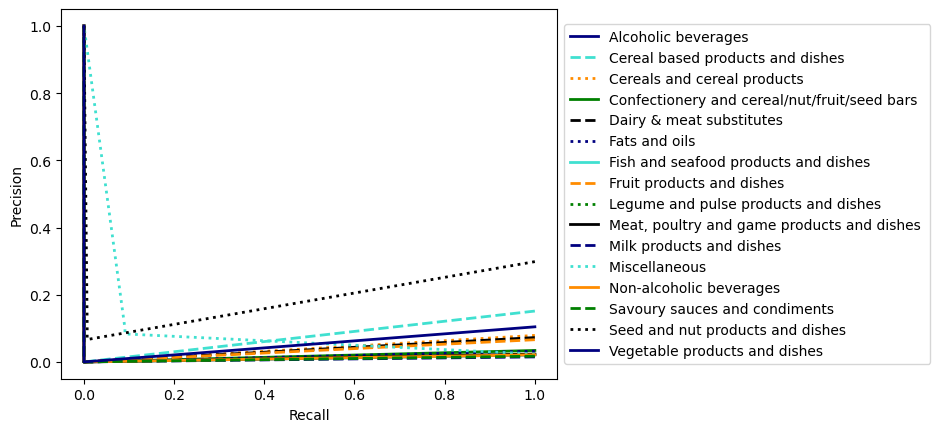
\includegraphics[width=\textwidth]{knn-precision-recall}
        \caption{Precision Recall Curve of Each Class With KNN K = 2}
        \label{fig:knn-precision-recall}
    \end{figure}

    \begin{figure}[h]
        \centering
        \begin{minipage}{0.5\textwidth}
            \centering
            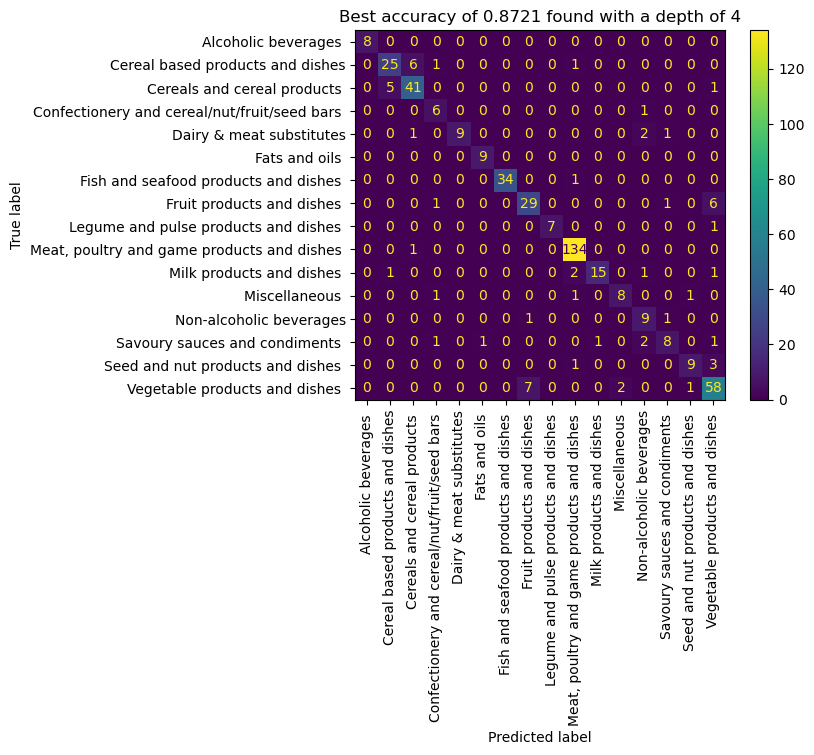
\includegraphics[width=\textwidth]{knn-conf-nopca} % first figure itself
            \caption{KNN Confusion Matrix, no PCA}
            \label{fig:knn-conf-nopca}
        \end{minipage}\hfill
        \begin{minipage}{0.5\textwidth}
            \centering
            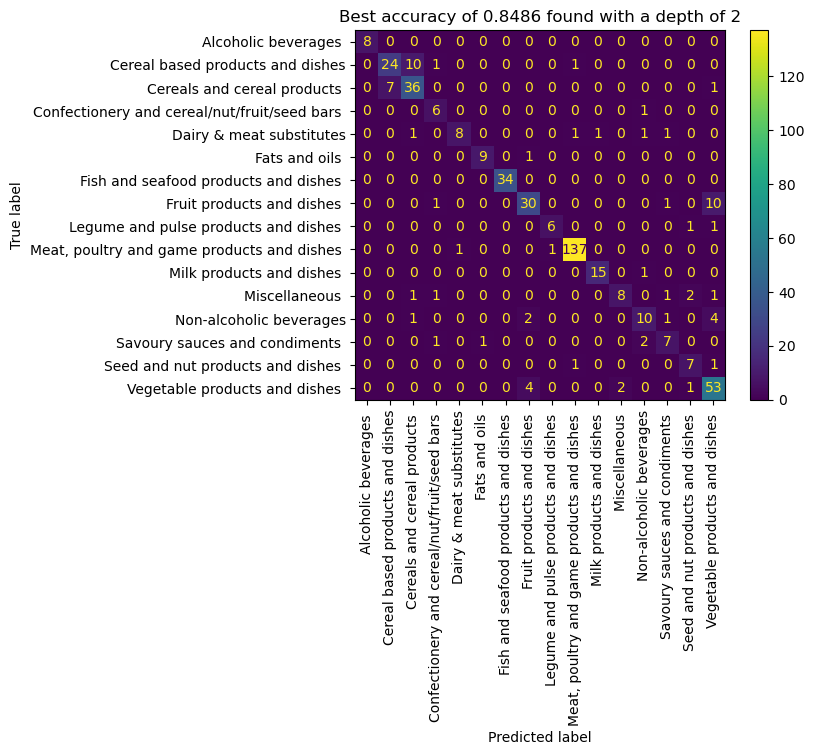
\includegraphics[width=\textwidth]{knn-conf-pca} % second figure itself
            \caption{KNN Confusion Matrix, PCA}
            \label{fig:knn-conf-pca}
        \end{minipage}
    \end{figure}

    \clearpage
    \section{Random Forest Classifier}
    \subsection{Training}
    When we are adjusting the hyperparameters to train a random forest classifier, much akin
    to the KNN, we only have one variable to change, in this case it is the depth with 
    which we search along a decision tree. Our random forest classifier makes several devision
    trees of a certain depth, and chooses them at random to produce a model which can predict
    the class based on the features.
    \\
    \\
    Our random forest classifiers, as trained below in figures \ref{fig:random-forest-nopca} and
    \ref{fig:random-forest-pca}, get very accurate quite quickly. However, in converse to
    the KNN, we stay consistently accurate and do not lose any ability as we increase the
    depth. Simply plateauing around 0.9 accuracy for both models. 

    \begin{figure}[h]
        \centering
        \begin{minipage}{0.45\textwidth}
            \centering
            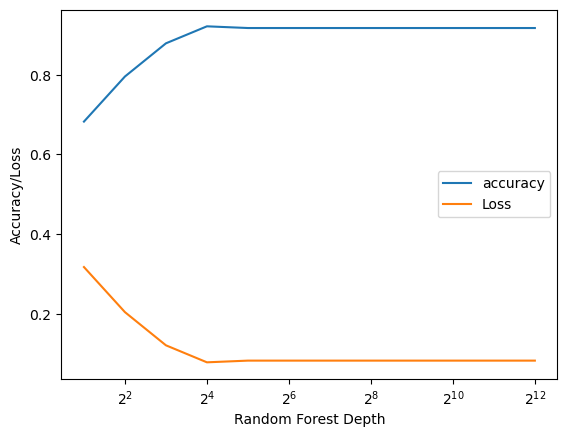
\includegraphics[width=0.9\textwidth]{random-forest-nopca} % first figure itself
            \caption{Random forest model test loss and accuracy vs depth. No PCA}
            \label{fig:random-forest-nopca}
        \end{minipage}\hfill
        \begin{minipage}{0.45\textwidth}
            \centering
            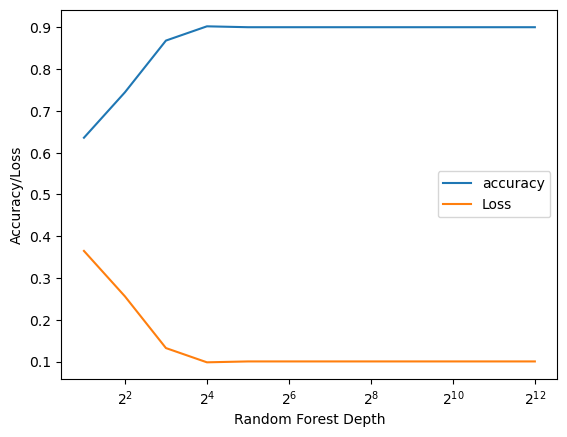
\includegraphics[width=0.9\textwidth]{random-forest-pca} % second figure itself
            \caption{Random forest model test loss and accuracy vs depth. Using PCA}
            \label{fig:random-forest-pca}
        \end{minipage}
    \end{figure}

    This is likely due to the difference in nature of the two models. Since KNN has the ability
    to become confused by too much data, we see that drop off in accuracy as we increase k.
    However, our random forests simply make more decisions as we increase the depth. If the
    model is already doing the best it can, the decision can simply be to return whatever it
    is currently guessing for every decision afterwards. This means we get no loss in clarity
    for higher depth.

    \subsection{Results}
    When looking at the precision recall curves in figure \ref{fig:random-forest-precision-recall},
    we can see that we have a significantly curvier graph. There is far more going on in each curve.
    This is a sign that the model is having a bit more of a handle on what the relationship between the
    features and the classes is. However, the actual values are not much better than those attained from
    KNN.
    \\
    \\
    The confusion matrices between the two models (pca vs no pca) in figures \ref{fig:random-forest-conf-nopca}
    and \ref{fig:random-forest-conf-pca}, we see that, once again, the model that doesn't use PCA has slightly
    higher accuracy. This time, though, the model which is not using PCA does not reach this accuracy any
    slower than the model which does.

    \clearpage
    \subsection{Figures}
    \begin{figure}[h]
        \centering
        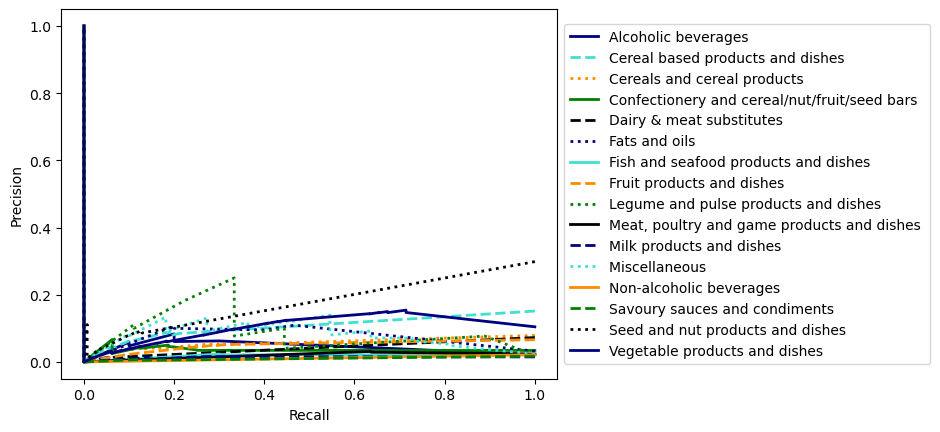
\includegraphics[width=\textwidth]{random-forest-precision-recall}
        \caption{Precision Recall Curve of Each Class With Depth of 16}
        \label{fig:random-forest-precision-recall}
    \end{figure}

    \begin{figure}[h]
        \centering
        \begin{minipage}{0.48\textwidth}
            \centering
            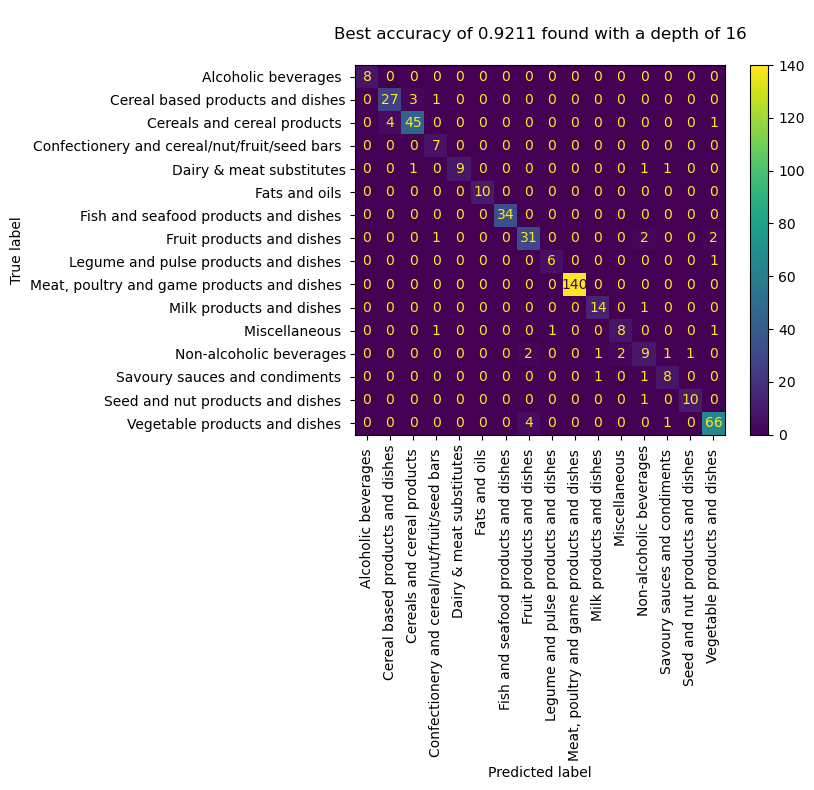
\includegraphics[width=\textwidth]{random-forest-conf-nopca} % first figure itself
            \caption{Random Forest Confusion Matrix, no PCA}
            \label{fig:random-forest-conf-nopca}
        \end{minipage}\hfill
        \begin{minipage}{0.48\textwidth}
            \centering
            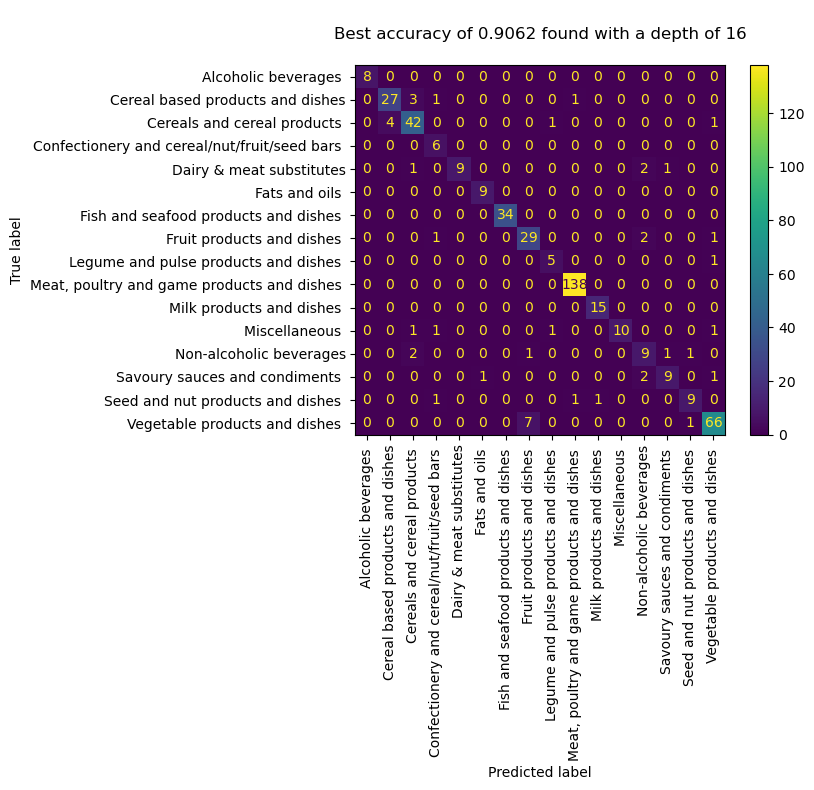
\includegraphics[width=\textwidth]{random-forest-conf-pca} % second figure itself
            \caption{Random Forest Confusion Matrix, PCA}
            \label{fig:random-forest-conf-pca}
        \end{minipage}
    \end{figure}

    \clearpage
    \section{Convolutional Neural Network Classifier}
    The previous two models used the scikit-learn library and had very simple setups. I simply passed them
    the train data, and they would train with whatever k or depth I chose. This next mode, a convolutional
    neural network (CNN), requires significantly more setup in order to get working.
    \\
    To see exact code done to create this model see the appendix, otherwise I will continue with a high level
    description.

    \subsection{Model Creation}
    To define our CNN, we define each step our model will perform to transform from our features, into the
    classes that we want out. In order to perform a convolution on this data, however, we need to introduce
    a channels dimension to our features. We do this using pytorchs unsqueeze method. Next we can start passing
    through our convolutional layers. I chose to have 3 convolutional layers in my model.
    \\
    \\
    After each convolution, we apply a relu filter, then max pooling, batch normalization, and a dropout.
    \\
    \\
    The relu filter is a sort of soft max for the activation of each neuron, this helps when using sparse
    data and propogating gradients.
    \\
    The pooling is then used to downsample the data, this works to reduce
    the dimensionality of the features since the convolution will have increased the dimensionality.
    \\
    Next, we apply a batch normalization, this works to normalize the data between 0 and 1, this helps
    to stabilize the information and introduce learnable parameters.
    \\
    Finally, we have a dropout layer. Typically, we can run into issues with convolution where the model
    is learning too well, typically it is overfitting to certain datapoints, and not learning the actual
    correlations. So we introduce a dropout layer, which will randomly
    delete weights and force the model to learn them again with a chance of dropout rate.
    \\
    \\
    After all of these steps have happened 3 times, for each of our convolutional layers, we flatten the features.
    This returns our data to be in the same form as when it went into the model, getting rid of our channel dimension.
    We can then pass this through 2 fully connected layers, with the first one using the same relu filter as the convolutions, 
    to finally get ourselves down to a shape equal to the number of classes.
    \\
    \\
    All of these steps require a lot of hyperparameter tuning about what sizes and shapes we transform the
    data into in order to learn efficiently and produce a final shape from which we can extract the predicted
    classes.

    \subsection{Train Loop}
    Next we need to define how we are going to fit our model to the data. Using pytorch lightning I am able
    to reduce the amount of code I need to write to make this happen, but the overall process is much the same.
    We extract the features and classes from our batch, we then predict the classes using the features, and return
    the loss from comparing our predicted classes to the actual class. 
    \\
    \\
    The loss function I chose was cross entropy loss.
    This is because this loss function is the most suited for multiclass problems, especially when there is high dimensionality.
    Cross entropy works by comparing the prediction to the actual in a way that returns probabilities of picking each
    class. This means that we can have a good balance between optimization, stability, and accuracy by encouraging
    the model to learn meaningful representations of the data.
    \\
    \\
    The steps that pytorch lightning allow me to not write is the backpropagation of the loss and zero grad
    through our weights. This is an important step which allows our model to do something meaningful with 
    the loss found as a result of this training. When we update the weights, we clear our gradients first, 
    then set them to new values based on the result of our loss function.
    \\
    \\
    We calculate the effect we are going to have on the actual weights of each component using our optimizer.
    For this model I have chosen the ADAM optimizer. Adam is considered a very aggressive and jack of all
    trades optimizer, this is because it is very good at learning almost any problem. Attempts with using
    the SGD optimizer, another popular optimizer, instead of adam resulted in significantly worse loss and
    accuracies. This is due to SGD not being adaptive to the data it receives, and just working off of it's 
    simple equations.
    \\
    \\
    After we do a single pass through a batch with our training dataset, we do a pass with our validation dataset.
    This pass happens almost identically to the training step, except with a subset of the train set that has been
    kept seperate, so there should be no leaking. This is like a mini test step where we validate that what we did 
    inside of our training step made sense in the context of the dataset as a whole.

    \subsection{Test Loop}
    After our model has been trained, we do a test loop. In this loop we go over an entirely unseen dataset called
    the train dataset. This information will not have been seen in any stage during training, and our model is no longer
    updating any of its weights, only logging the loss and accuracy.

    \subsection{Analysis of Result}
    Two models have been trained once again, comparing the effectiveness of PCA. 
    We observe that the train and validation loss for our cnn in figures \ref{fig:cnn-train-loss} and \ref{fig:cnn-val-loss}
    are very even. We have good loss that is steadily decreasing as our model trains. Our learning rate start at 0.001
    and a learning rate optimizer that lowers the learning rate as our model gets closer to convergence. This technique
    helps us so that as we approach the low point in our gradient descent, we can make sure that we don't accidentally
    step out of our global minima and into a local minima.
    \\
    \\
    At the end of training, we see the final accuracies of each model, we observe that the accuracy of the model with pca
    is slightly better than the model without pca, although not significantly. And, in fact, we see that the model with pca 
    took longer to train in more number of epochs. In fact, the pca model took about 20 minutes longer to train than the no pca model.
    And when we come down to the precision recall curves and confusion matrices in figures \ref{fig:cnn-nopca-prec}, \ref{fig:cnn-pca-prec},
    \ref{fig:cnn-nopca-conf-mat}, and \ref{fig:cnn-pca-conf-mat} we see that the model with pca actually has higher precision to high recall
    when compared to the model without PCA. So we have a tradeoff with our PCA increasing the time for our model to learn the information,
    but becoming a better model as a result.
    \\
    \\
    When comparing these models to our previous KNN and random forests, our overall accuracy isn't actually that much better than these models.
    Only sitting around 0.8, however, our precision recall curves are significantly better. We were able to reach this by varying the hidden layers
    and therefore the shape of our transformations on the model, as well as our adjustments to the learning rate and our choice of optimizers and loss function.

    \clearpage
    \subsection{Figures}
    \begin{figure}[h]
        \centering
        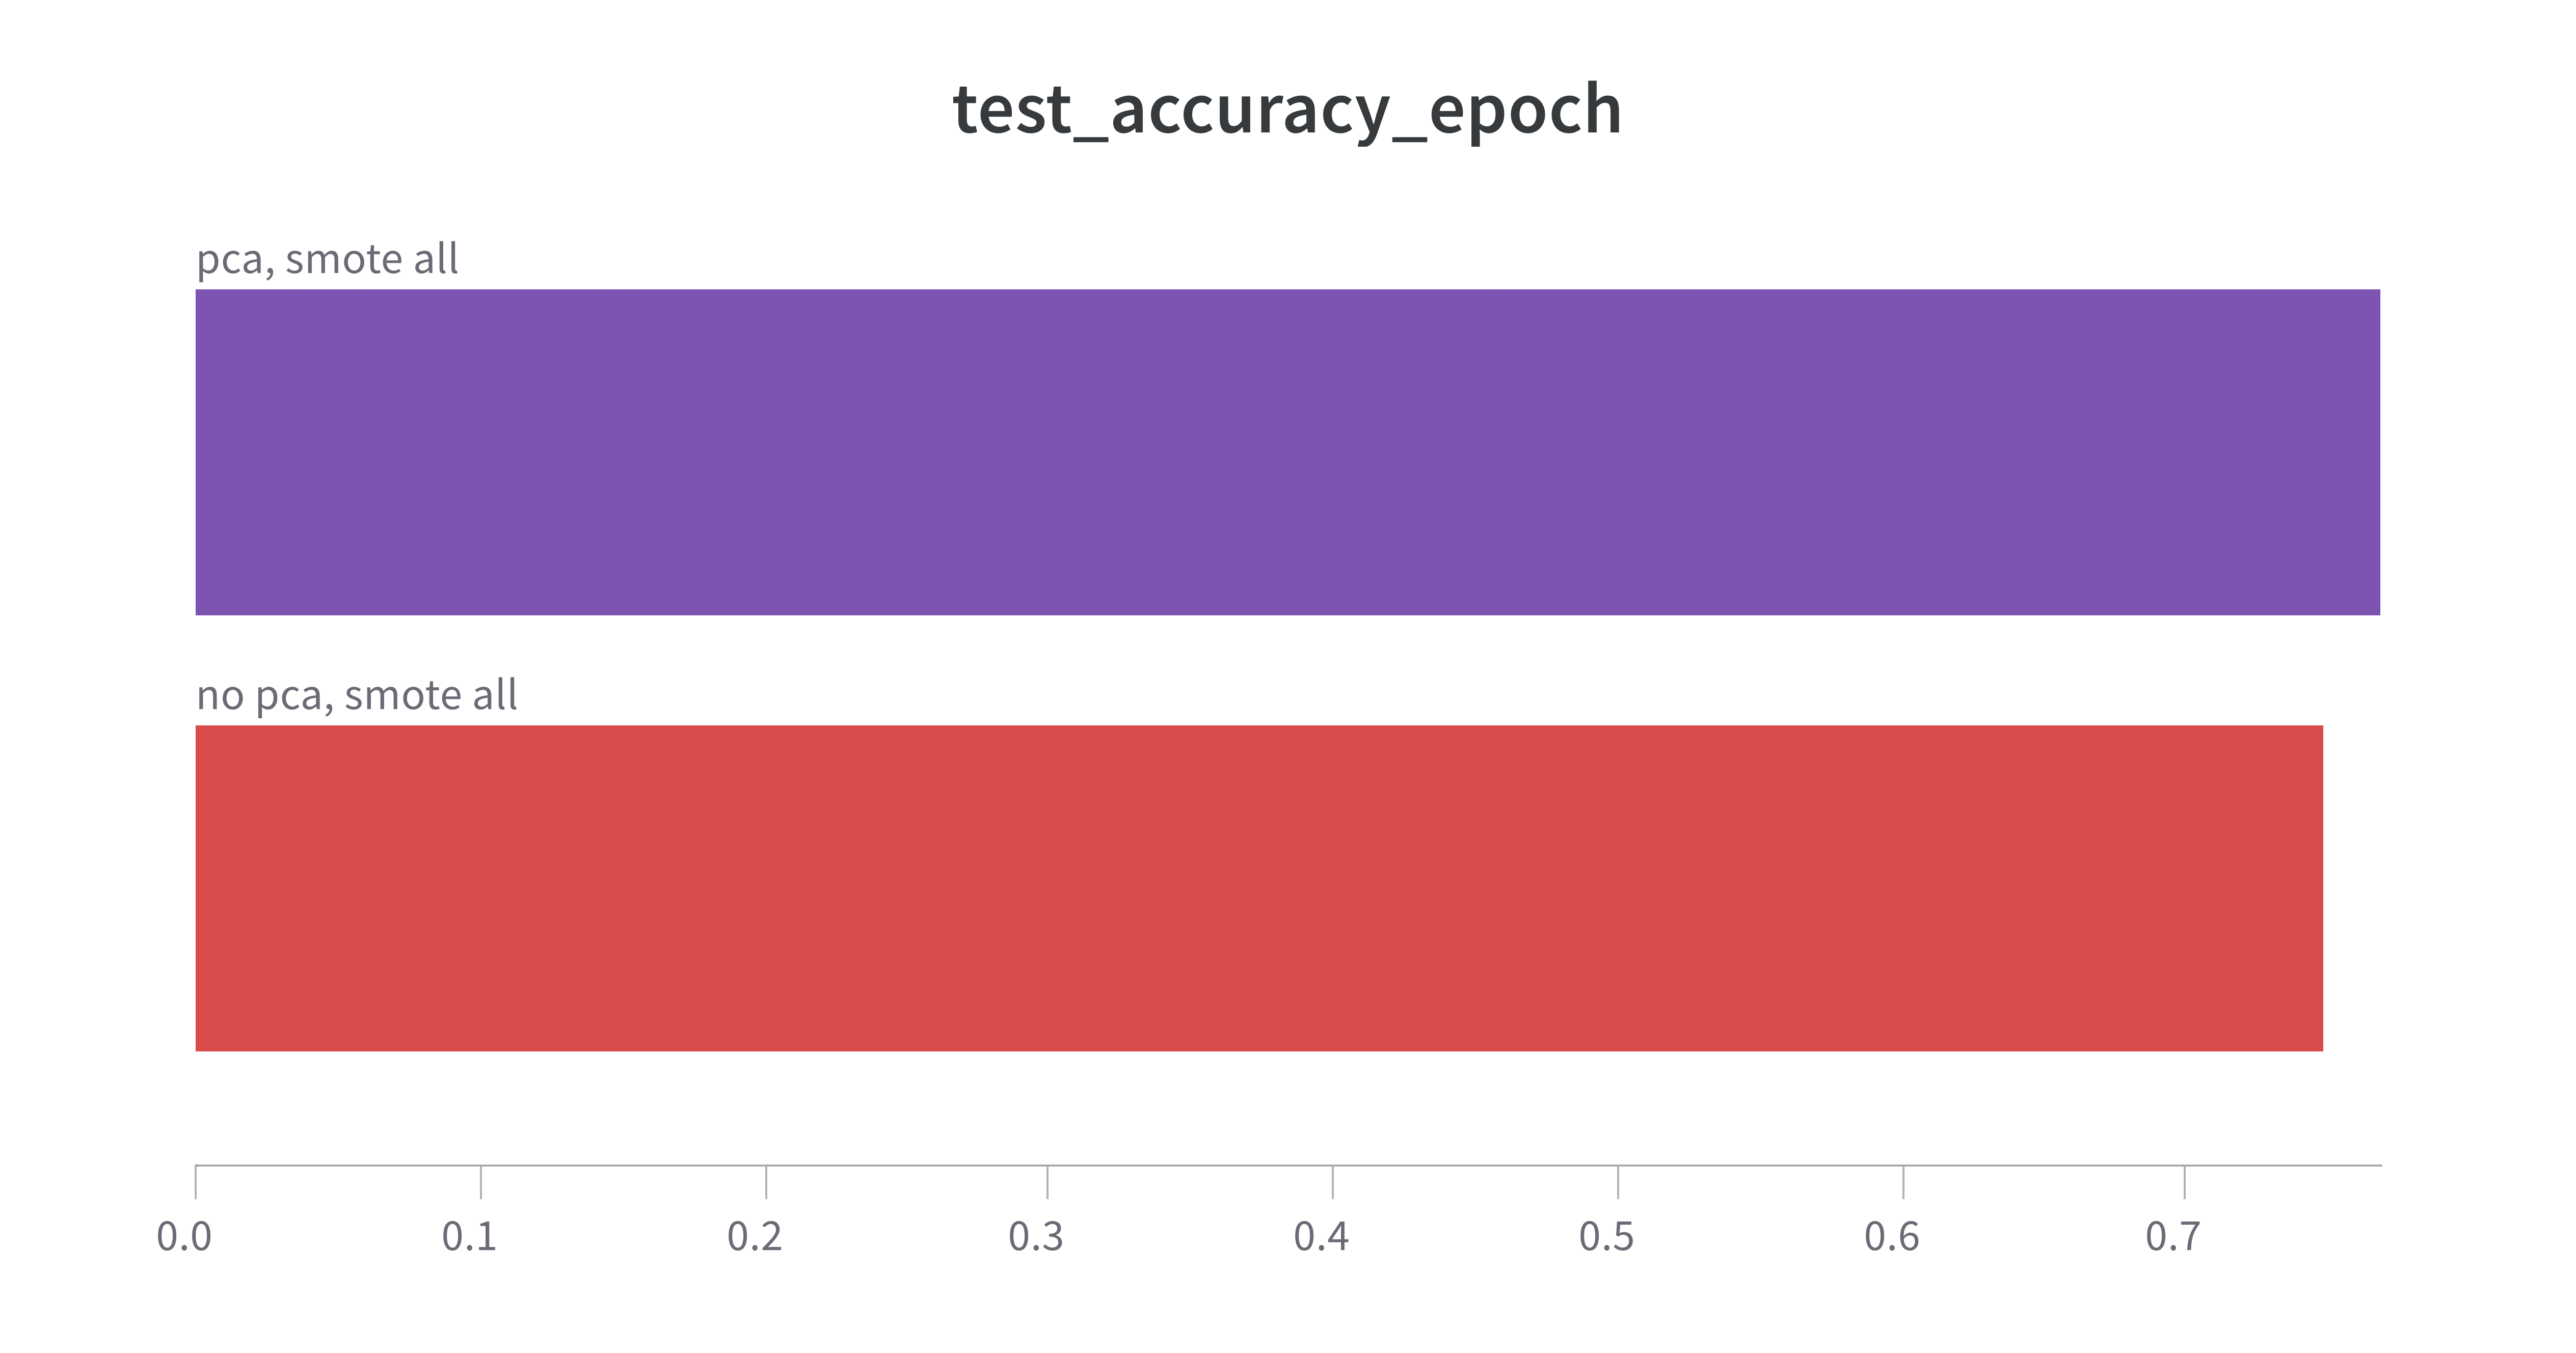
\includegraphics[height=0.3\textheight]{cnn-test-acc}
        \caption{CNN Accuracies}
        \label{fig:cnn-test-acc}
    \end{figure}

    \begin{figure}[h]
        \centering
        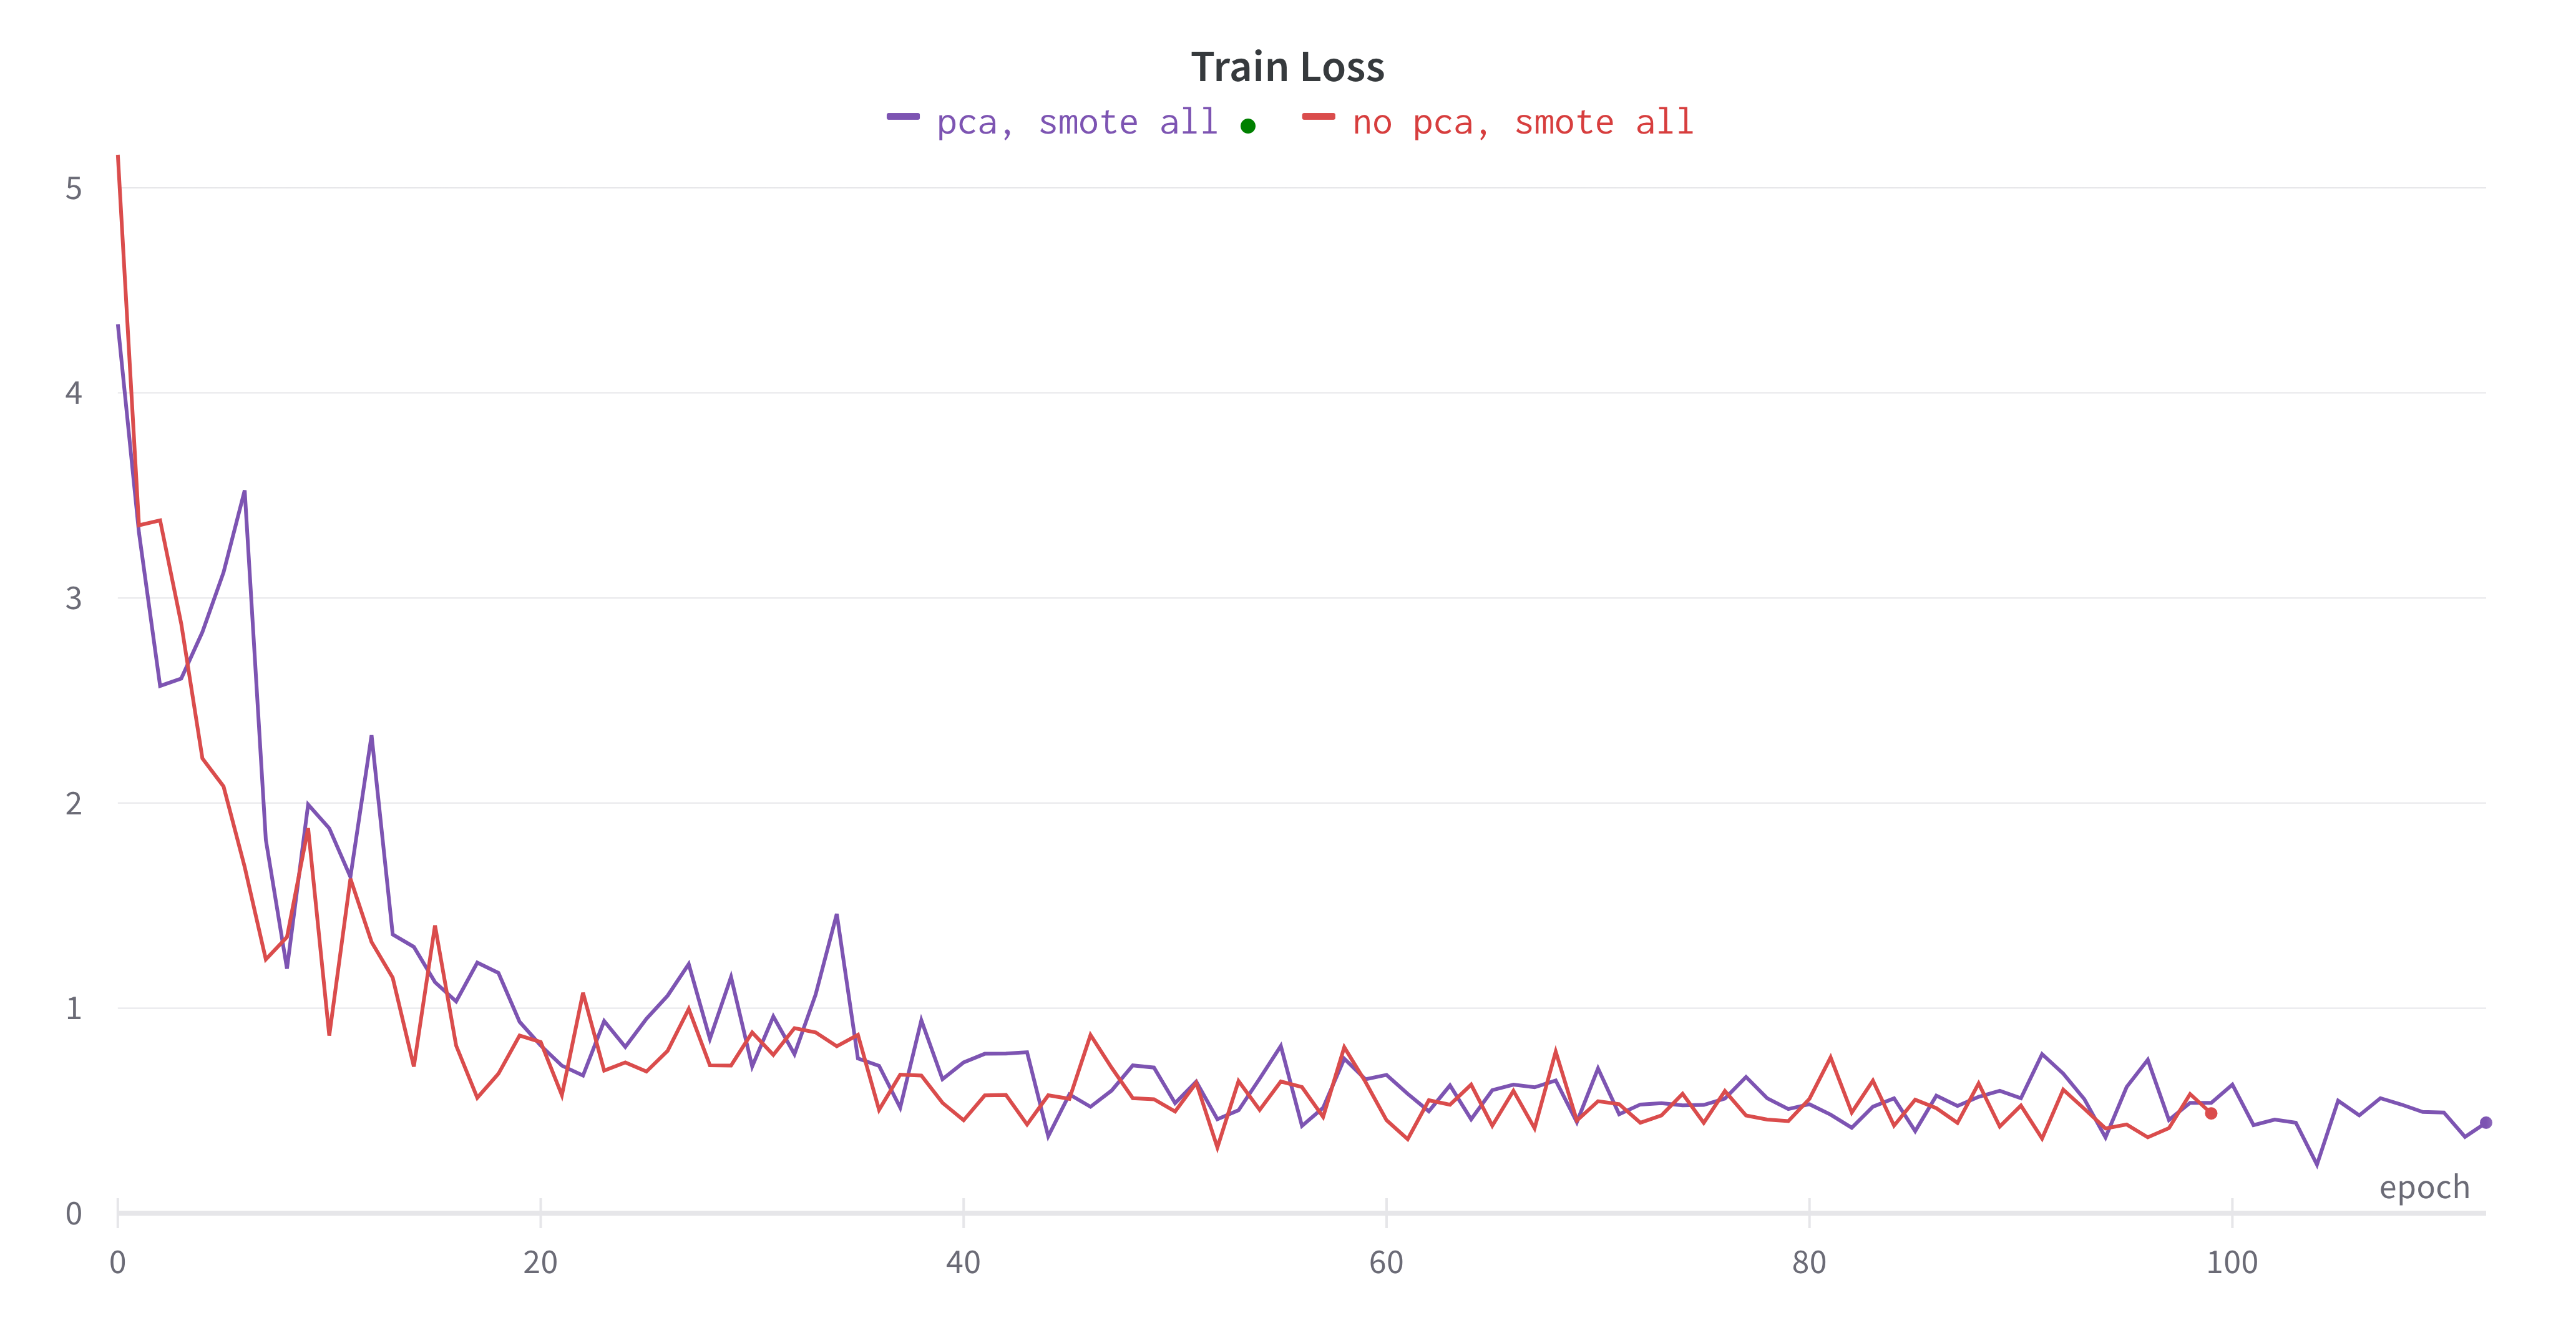
\includegraphics[height=0.3\textheight]{pca-train-loss}
        \caption{CNN Train Loss PCA vs no PCA}
        \label{fig:cnn-train-loss}
    \end{figure}

    \begin{figure}[h]
        \centering
        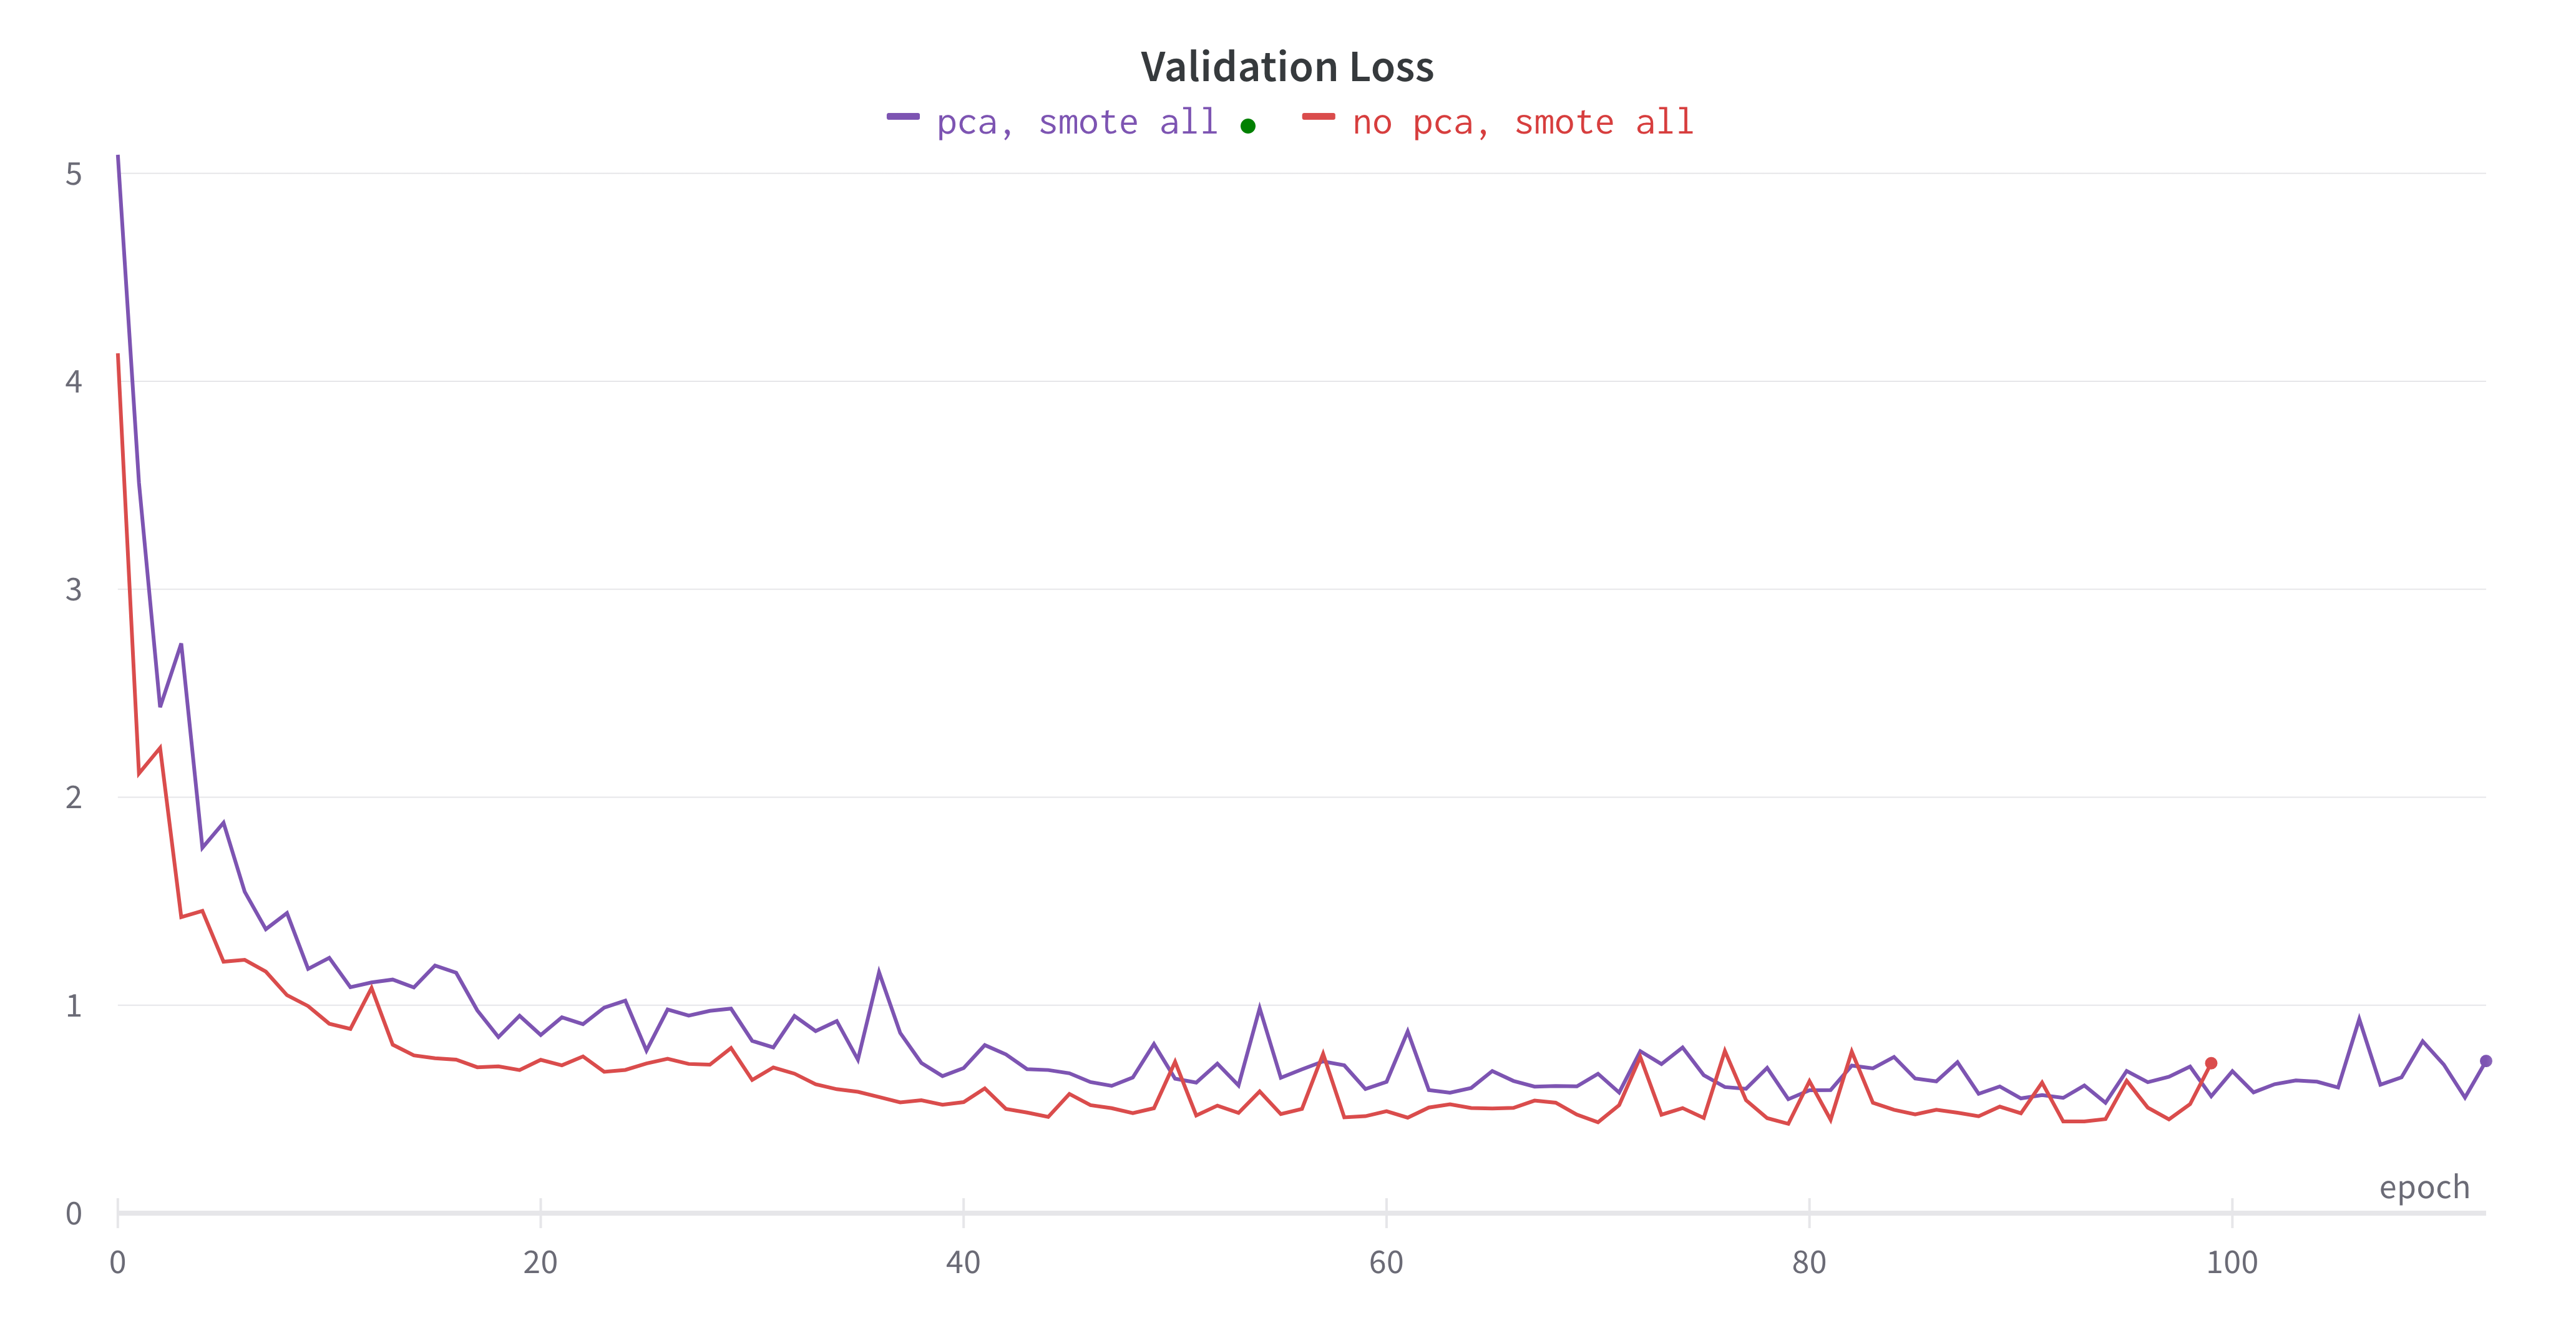
\includegraphics[height=0.3\textheight]{smote-all-val-loss}
        \caption{CNN Validation Loss PCA vs no PCA}
        \label{fig:cnn-val-loss}
    \end{figure}

    \begin{figure}[h]
        \centering
        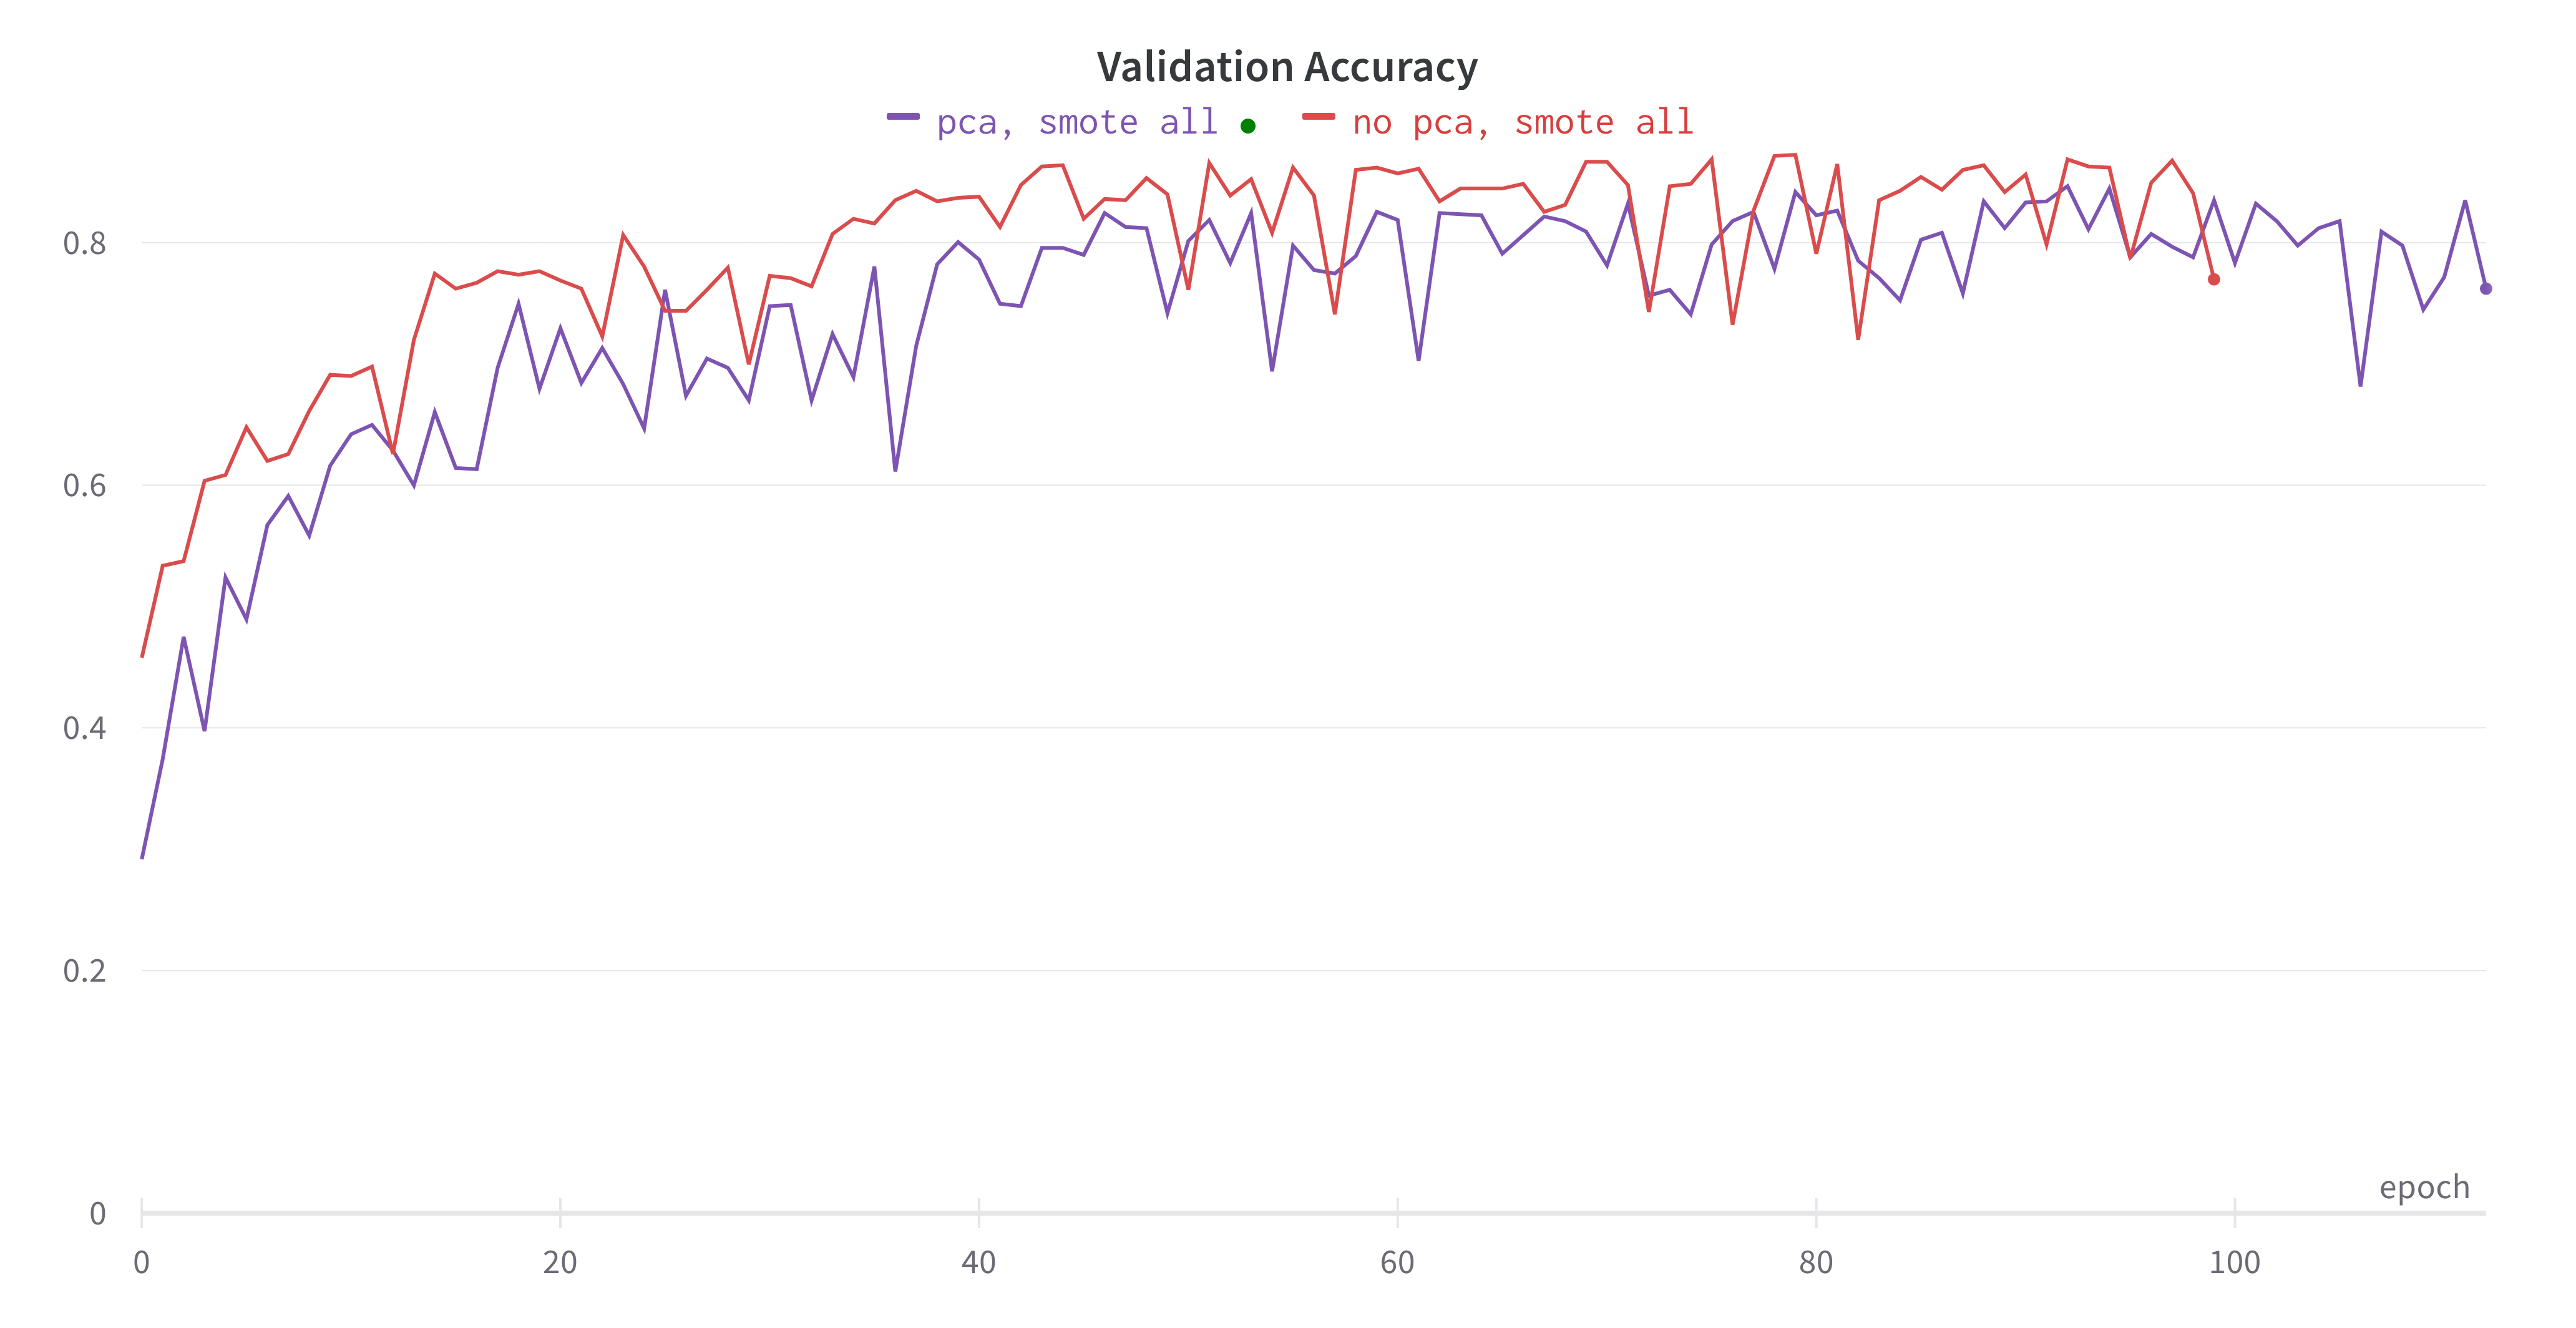
\includegraphics[height=0.3\textheight]{smote-all-val-acc}
        \caption{CNN Validation Accuracy PCA vs no PCA}
        \label{fig:cnn-val-acc}
    \end{figure}

    \begin{figure}[h]
        \centering

        \begin{minipage}{0.48\textwidth}
            \centering
            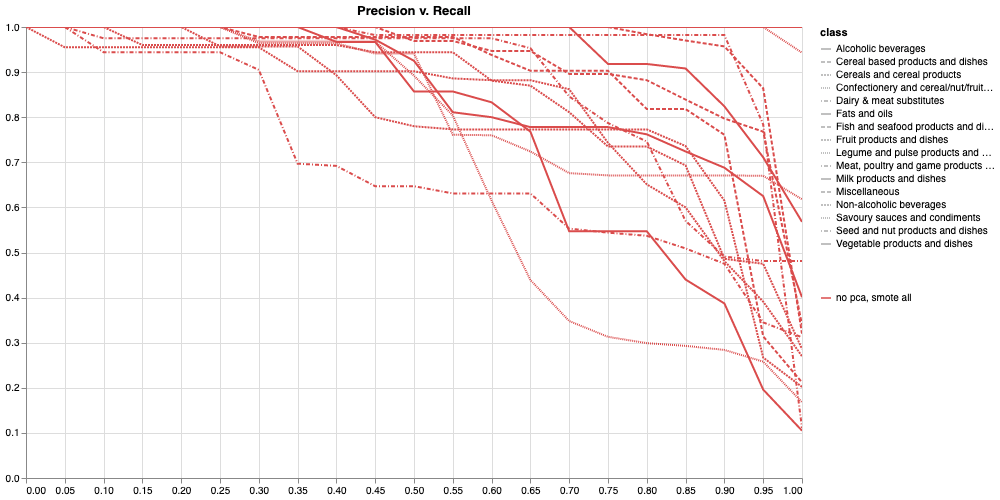
\includegraphics[width=\textwidth]{cnn-nopca-prec} % first figure itself
            \caption{CNN Precision Recall Curve, no PCA}
            \label{fig:cnn-nopca-prec}
        \end{minipage}\hfill

        \begin{minipage}{0.48\textwidth}
            \centering
            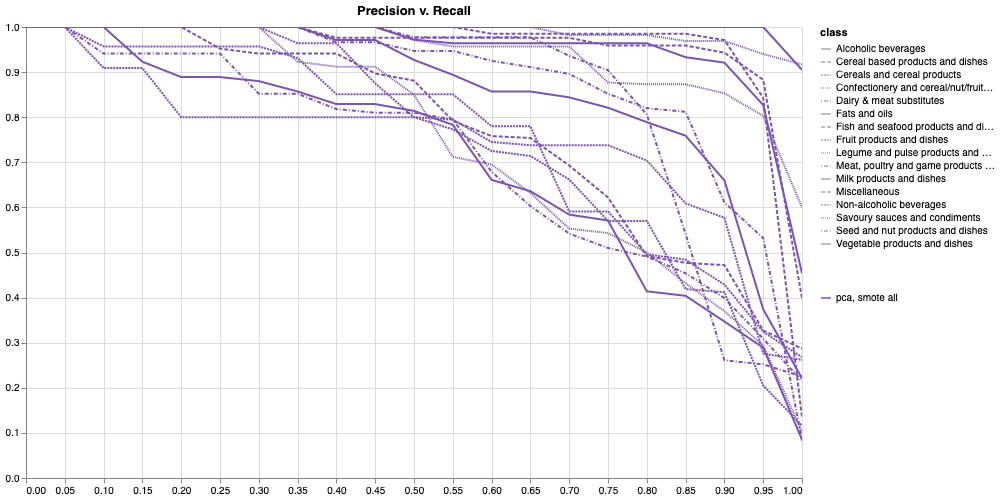
\includegraphics[width=\textwidth]{cnn-pca-prec} % second figure itself
            \caption{CNN Precision Recall Curve, PCA}
            \label{fig:cnn-pca-prec}
        \end{minipage}

    \end{figure}

    \begin{figure}[h]
        \centering

        \begin{minipage}{0.48\textwidth}
            \centering
            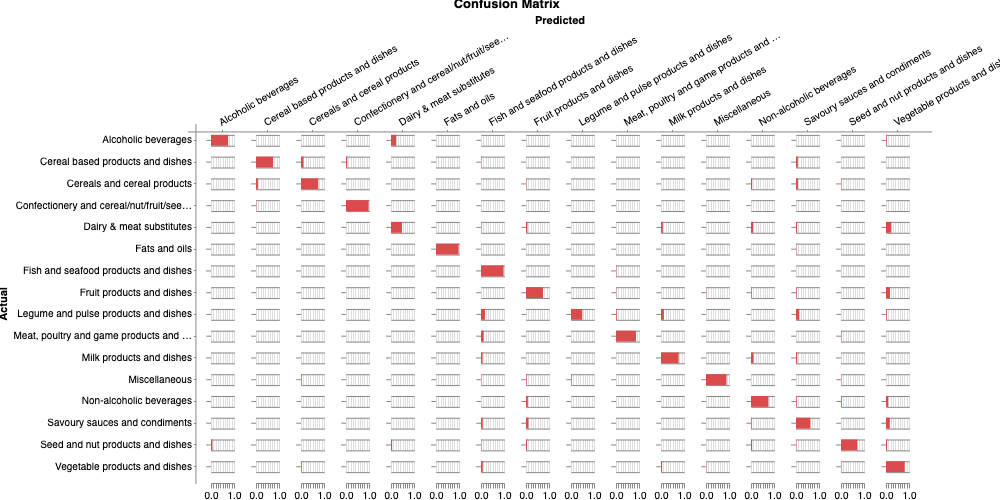
\includegraphics[width=\textwidth]{cnn-nopca-conf-mat} % first figure itself
            \caption{CNN Confusion Matrix, no PCA}
            \label{fig:cnn-nopca-conf-mat}
        \end{minipage}\hfill

        \begin{minipage}{0.48\textwidth}
            \centering
            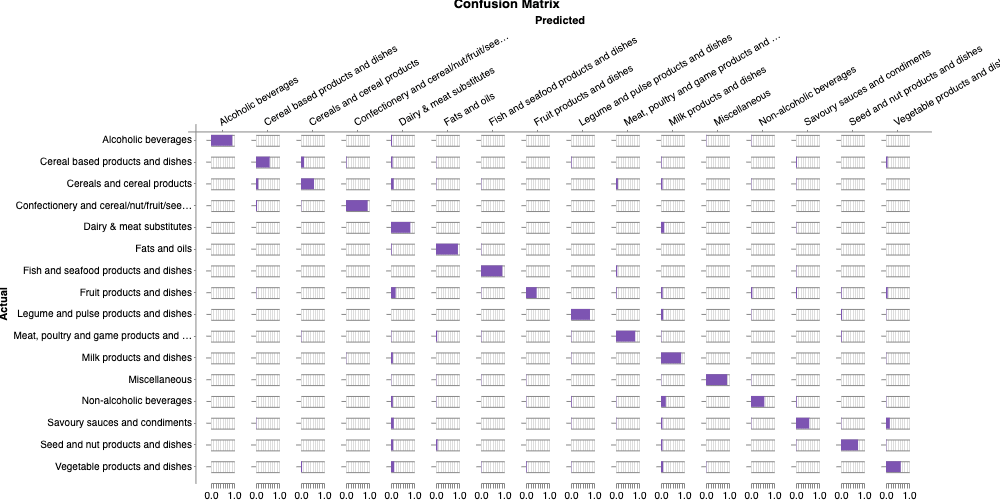
\includegraphics[width=\textwidth]{cnn-pca-conf-mat} % second figure itself
            \caption{CNN Confusion Matrix, PCA}
            \label{fig:cnn-pca-conf-mat}
        \end{minipage}

    \end{figure}

    \clearpage
    \section{Conclusion}
    To conclude, when comparing these different models, we see vastly different approaches to the same problem.
    Our KNN simply looked at how the data was grouped in n-dimensional space and made a best guess based on how many neighbours
    were of the same class. The random forests made a group of decision trees and selected one at random which would make decisions
    based on a previous decision and the ones to follow. Our CNN created a deep net of neurons with convolutional layers and manipulated the
    dimensionality of the features until discovering the classes with the final dimensionality.
    \\
    \\
    Given how significantly better our CNN is at precision and recall than the KNN and random forests, we see just how
    highly dimensional our dataset is. Given a CNN is typically used for image data which is another factor of dimensionality on top of this.
    \\
    \\
    The benefits of training a CNN do come at a cost however, this cost comes in the setup and training time.
    When training the KNN and random forests, each run took only a couple seconds per each variation in the hyperparameters (k and depth respectively).
    The CNN however, took around 40 minutes for each adjustment to the hyperparameters. This increases the time to train and find the best model significantly.
    \\
    \\
    We can make this easier for ourselves using techniques like an early stopping callback which checks a variable (such as loss or accuracy) and if no improvement
    has happened in some amount of epochs, then we cancel the model. This can help avoid being stuck in a run that is getting nowhere, as well as avoiding overfitting
    by stopping the model at a certain maximum accuracy.
    \\
    \\
    For all the variation in how I am training this model, I needed to create a model which could vary to different dimensions of input. This involved having ternary
    statements to resize the features if needed to reintroduce a dimension in order for pooling to happen and perform a proper down sampling. We also needed
    to use an adaptive max pooling. This has produced a model which is highly adaptable and could be pointed at problems with lots of features but only along 1 dimension.
    

    \clearpage
    \section{Appendix}
    \subsection{PyTorch CNN}
    \begin{minted}
        [
        frame=lines,
        framesep=2mm,
        baselinestretch=1.2,
        bgcolor=LightGray,
        fontsize=\footnotesize,
        linenos
        ]
        {python}
class CNNClassifier(pl.LightningModule):
    def __init__(self, input_size, hidden_size, num_classes, lr, dropout_rate=0.5):
        super(CNNClassifier, self).__init__()
        # Calculate the number of channels for each convolutional layer
        conv1_channels = max(1, hidden_size // 8)
        conv2_channels = max(1, hidden_size // 4)
        conv3_channels = max(1, hidden_size // 2)
        self.conv1 = nn.Conv1d(in_channels=1, out_channels=conv1_channels, 
                kernel_size=2, stride=2)
        self.conv2 = nn.Conv1d(in_channels=conv1_channels, 
                out_channels=conv2_channels, kernel_size=2, stride=2)
        self.conv3 = nn.Conv1d(in_channels=conv2_channels,
                out_channels=conv3_channels, kernel_size=2, stride=2)
        self.pool = nn.AdaptiveMaxPool1d(output_size=1)
        self.dropout = nn.Dropout(dropout_rate)
        self.batchnorm1 = nn.BatchNorm1d(conv1_channels)
        self.batchnorm2 = nn.BatchNorm1d(conv2_channels)
        self.batchnorm3 = nn.BatchNorm1d(conv3_channels)
        self.fc1 = nn.Linear(conv3_channels, conv1_channels)
        self.fc2 = nn.Linear(conv1_channels, num_classes)
        self.lossfn = nn.CrossEntropyLoss()
        nn.init.xavier_uniform_(self.fc1.weight) # Initialize fc1 weights
        nn.init.xavier_uniform_(self.fc2.weight) # Initialize fc2 weights
        self.learning_rate = lr

    def forward(self, x):
        x = x.unsqueeze(1)  # Add a channel dimension for 1D convolution
        x = F.relu(self.conv1(x))
        x = self.pool(x)
        x = self.batchnorm1(x)
        x = self.dropout(x)
        x = x.expand(x.shape[0], x.shape[1], 2) if x.shape[-1] < 2 else x
        x = F.relu(self.conv2(x))
        x = self.pool(x)
        x = self.batchnorm2(x)
        x = self.dropout(x)
        x = x.expand(x.shape[0], x.shape[1], 2) if x.shape[-1] < 2 else x
        x = F.relu(self.conv3(x))
        x = self.pool(x)
        x = self.batchnorm3(x)
        x = self.dropout(x)
        x = x.view(x.size(0), -1)  # Flatten the tensor
        x = F.relu(self.fc1(x))
        x = self.fc2(x)
        return x
    \end{minted}
    
    \subsection{CNN train, val, test loops and optimisation setup}
    \begin{minted}
        [
        frame=lines,
        framesep=2mm,
        baselinestretch=1.2,
        bgcolor=LightGray,
        fontsize=\footnotesize,
        linenos
        ]
        {python}

    def training_step(self, batch, batch_idx):
        x, y = batch
        # Forward pass
        y_hat = self(x)
        # Calculate loss
        loss = self.lossfn(y_hat, y)
        # Log accuracy and loss (optional)
        self.log("train_loss", loss, prog_bar=True)

        return loss

    def validation_step(self, batch, batch_idx):
        x, y = batch
        y_hat = self(x)
        loss = self.lossfn(y_hat, y)
        _, predicted = torch.max(y_hat, dim=1)
        # Calculate accuracy
        accuracy = torch.sum(predicted == y).item() / len(y)
        self.log("val_acc", accuracy, prog_bar=True, on_epoch=True)
        self.log("val_loss", loss, on_step=True, on_epoch=True, prog_bar=True, logger=True)

    def test_step(self, batch, batch_idx):
        x, y = batch
        y_hat = self(x)
        loss = self.lossfn(y_hat, y)
        self.log("test_loss", loss, on_step=True, on_epoch=True, prog_bar=True, 
                logger=True)
        _, predicted_labels = torch.max(y_hat, 1)
        accuracy = torch.sum(predicted_labels == y).item() / len(y)
        self.log("test_accuracy", accuracy, on_step=True, on_epoch=True, prog_bar=True, 
                logger=True)

    def configure_optimizers(self):
        optimizer = torch.optim.Adam(self.parameters(), lr=self.learning_rate)
        scheduler = torch.optim.lr_scheduler.StepLR(optimizer=optimizer, step_size=35, 
                gamma=0.1, verbose=True)
        scheduler_dict = {
            "scheduler": scheduler,
            "interval": "epoch",
            "monitor": "val_loss",
        }

        return [optimizer], [scheduler_dict]

    \end{minted}

    \subsection{Model and Training Initialization}
    \begin{minted}
        [
        frame=lines,
        framesep=2mm,
        baselinestretch=1.2,
        bgcolor=LightGray,
        fontsize=\footnotesize,
        linenos
        ]
        {python}

    # Data setup
    batch_size = 64
    train_loader = DataLoader(train_dataset, batch_size=batch_size, shuffle=True)
    val_loader = DataLoader(val_dataset, batch_size=batch_size)
    test_loader = DataLoader(test_dataset, batch_size=batch_size)
    
    input_size = MLP_X_train.shape[1]
    hidden_size = 8192
    num_classes = len(new_df["Classification_seq"].unique())
    lr = 1e-3
    EPOCHS = 200
    
    model = CNNClassifier(input_size=input_size, hidden_size=hidden_size, 
            num_classes=num_classes + 1, lr=lr)

    wandb.init(
        project="COMP4702",
        config={
            "learning_rate": lr,
            "batch_size": batch_size,
            "hidden_size": hidden_size,
            "input_size": input_size,
            "num_classes": num_classes,
            "model_architecture": "CNN",
            "dataset": "Nutrition",
        },
    )
    
    wandb_logger = WandbLogger(project="Nutrition_Assignment_")
    # Create the EarlyStopping and LearningRateMonitor callbacks
    early_stopping = EarlyStopping(
        monitor="val_acc", mode="max", patience=20, stopping_threshold=0.95
    )
    lr_monitor = LearningRateMonitor(logging_interval="step")
    metrics_callback = MetricsCallback(classes=list(new_df["Classification_seq"].unique()))
    callback_list: list[Callback] = [early_stopping, lr_monitor, metrics_callback]
    
    # Trainer setup
    trainer = pl.Trainer(max_epochs=EPOCHS, logger=wandb_logger, callbacks=callback_list)
    
    # Model training
    trainer.fit(model=model, train_dataloaders=train_loader, val_dataloaders=val_loader)
    
    # Model testing
    trainer.test(model, test_loader)
    \end{minted}
\end{document}